\documentclass[11pt]{article}
\usepackage[letterpaper,top=2cm,bottom=2cm,left=2cm,right=2cm,marginparwidth=1.75cm]{geometry}

 % Useful packages 
\usepackage{hyperref}
\usepackage{biblatex}
\addbibresource{Bib.bib}
\usepackage{mathtools}
\DeclarePairedDelimiterXPP\BigOSI[2]%
  {\mathcal{O}}{(}{)}{}%
  {\SI{#1}{#2}}

\usepackage{amsmath}
\usepackage{amssymb}
\usepackage{empheq}
\usepackage[most]{tcolorbox}
\usepackage{amsmath}
\usepackage{mathrsfs}
\usepackage[utf8]{inputenc}
\usepackage{graphicx}
\usepackage{float}
\usepackage{parskip}
\usepackage{comment}
\usepackage{mhchem}
 \usepackage{tabularx}
 \usepackage{titling}
  \usepackage[explicit]{titlesec}
\usepackage{fancyhdr}
\setlength{\droptitle}{3em} 

\title{Galactic Structure}
\author{Thomas Brosnan}
\date{Notes taken in Professor Evan Keane's class, Michaelmas Term 2023}

    
\numberwithin{equation}{section}

\newtcbox{\mymath}[1][]{%
    nobeforeafter, math upper, tcbox raise base,
    enhanced, colframe=blue!30!black,
    colback=blue!30, boxrule=1pt,
    #1}
 \newenvironment{bux}
    {
    \empheq[box=\tcbhighmath]{align}
   }{
    \endempheq
    }
    \newenvironment{bux*}
    {
    \empheq[box=\tcbhighmath]{align*}
   }{
    \endempheq
    }
\newcommand{\hsp}{\hspace{8pt}}

\newcommand*{\sectionFont}{%
  \LARGE\bfseries
}


\makeatletter
\let\Title\@title % Copy the title to a new command
\makeatother

%change this RGB value to change the section background colour 
\definecolor{mycolor1}{RGB}{74, 241, 130}
\colorlet{SectionColour}{mycolor1}
%subsection background colour 
\definecolor{mycolor2}{gray}{0.8}
\colorlet{subSectionColour}{mycolor2}
%subsubsection background colour 
\definecolor{mycolor3}{RGB}{255,255,255}
\colorlet{subsubSectionColour}{mycolor3}

\begin{document}

\maketitle

\newpage

\tableofcontents
% For \section
 \titleformat{\section}[block]{\sectionFont}{}{0pt}{%
 \fcolorbox{black}{SectionColour}{\noindent\begin{minipage}{\dimexpr\textwidth-2\fboxsep-2\fboxrule\relax}\thesection  \hsp #1 {\strut} \end{minipage}}}
% For \subsection
 \titleformat{\subsection}[block]{\bfseries}{}{0pt}{%
 \fcolorbox{black}{subSectionColour}{\noindent\begin{minipage}{\dimexpr\textwidth-2\fboxsep-2\fboxrule\relax}\thesubsection  \hsp #1 {\strut} \end{minipage}}}
% For \section*
 \titleformat{name=\section, numberless}[block]{\sectionFont}{}{0pt}{%
 \fcolorbox{black}{SectionColour}{\noindent\begin{minipage}{\dimexpr\textwidth-2\fboxsep-2\fboxrule\relax} #1 {\strut} \end{minipage}}}
  % For \subsection*
 \titleformat{name=\subsection, numberless}[block]{\bfseries}{}{0pt}{%
 \fcolorbox{black}{subSectionColour}{\noindent\begin{minipage}{\dimexpr\textwidth-2\fboxsep-2\fboxrule\relax} #1 {\strut} \end{minipage}}}
 % For \subsubsection
 \titleformat{\subsubsection}[block]{\bfseries}{}{0pt}{%
 \fcolorbox{black}{subsubSectionColour}{\noindent\begin{minipage}{15cm}\thesubsubsection \hsp #1 {\strut} \end{minipage}}}
  % For \subsubsection*
 \titleformat{name=\subsubsection, numberless}[block]{\bfseries}{}{0pt}{%
 \fcolorbox{black}{subsubSectionColour}{\noindent\begin{minipage}{15cm} #1 {\strut} \end{minipage}}}
\newpage
%header 
\pagestyle{fancy}
\fancyhf{} % Clear all header and footer fields
\fancyhead[L]{\Title}
\fancyhead[R]{\nouppercase{\leftmark}}
\fancyfoot[C]{-~\thepage~-}
\renewcommand{\headrulewidth}{1pt}


\normalsize
\newpage
\tcbset{highlight math style={boxsep=5mm,colback=red!0!blue!0!green!0!}}

\section{Types of Galaxies}

\subsection{Elliptical:} 
\begin{itemize}
    \item Surprisingly elliptical in shape, They have no spiral arms and no disc structure. 

Very little cool gas and dust, and thus not a lot of star formation.

They are denoted with an "$E\eta$" in the Hubble classification sequence where $\eta$ is the corresponding ellipticity , which is defined as 
\begin{empheq}[box=\tcbhighmath]{equation}
\begin{split}
    \eta = 1- \frac{b}{a}
    \end{split}
\end{empheq}
Where $a$ and $b$ are the major and minor axes respectively. 

It should be noted that galaxy types are based on their optical appearance and they make look different when inspected in different bands. 
\end{itemize}

\subsection{Spiral Galaxies}
\begin{itemize}
\item Visible spiral arms, have an obvious ISM (inter stellar medium) with gas and dust. 

Young "blue" stars present, i.e. star formation ongoing. 
These galaxies are denoted with an "$S$" in the Hubble classification. 
\end{itemize}

\subsection{Lenticular}
\begin{itemize}
    \item Lenticular galaxies are intermediate morphologically, i.e. they are neither elliptical nor spiral.

They are disc galaxies with a bulge but no spiral arms and little star formation. 
They are denoted with an $S0$ in the Hubble classification. 
\end{itemize}

\subsection{Hubble sequence}
\begin{itemize}
    \item Name given to the classification of galaxies, the order and use of the word sequence would imply that the galaxies follow some sort of time evolution between the different types, but this is not the case. 
\end{itemize}


\begin{figure}[H]
\centering
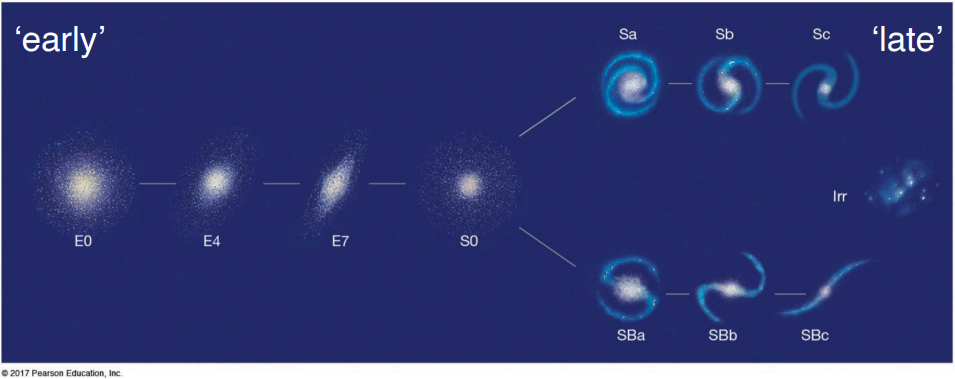
\includegraphics[width=0.7\textwidth]{Hubble sequence.png}
\caption{\label{fig:2}\emph{Hubble sequence}}
\end{figure}

\subsection{Galactic coordinates} 
\begin{itemize}
\item There are multiple coordinates used to describe positions of objects in the Milky way. 

There are the $(x,y,z)$ , that have the origin at the center of the Galaxy and the Sun $8$ Kpc up the y axis.

There are also the angular coordinates denoted $(gl,gb)$, l for longitude and b for latitude. For these the Sun is origin. 
\end{itemize}

\subsection{Dust}
\begin{itemize}
    \item The Milky is $\approx 1\%$ dust and $99 \% $ gas, but the dust can be quite impact. 
This is due to the size of the dust particles. The dust particles have sizes $a \leq 1 \mu m$, meaning they efficiently absorb and scatter radiation with $\lambda \leq a$, thus blue light is scattered and infrared is let through. 

The spectral radiance (or specific intensity) $I_{\lambda}$ changes infinitesimally when traversing a distance $ds$, and in a manner directly proportional to the incident 
$I_{\lambda}$. This means that:
\begin{empheq}[box=\tcbhighmath]{equation}
\begin{split}
    \frac{dI_{\lambda}}{ds} = -\kappa_{\lambda} \rho I_{\lambda}
\end{split}
\end{empheq}
Here, $\kappa_{\lambda}$ is the absorption coefficient, i.e. the opacity of the medium, $\rho$ is the density and the subscript $\lambda$ are there to remind us that this all depends of the wavelength of the light involved. 
The above equation can then be solved, resulting in: 
\begin{empheq}[box=\tcbhighmath]{equation}
\begin{split}
    I_{\lambda} = I_{\lambda,0} e^{-\int_0^s\kappa_{\lambda}\rho ds}
\end{split}
\end{empheq}
This exponent is known as the optical depth, $\tau_{\lambda}$. The optical depth is the number of mean free paths to which emission can traverse.


\end{itemize}

\subsection{Star distribution} 
\begin{itemize}
    \item By measuring the the velocities and positions of billions of stars accurately with Gaia, we can obtain equations for the distribution of stars in the Milky way. For this we have two formulas one for radial density and one for vertical out of the galactic plane density, thus the number of stars follow the following distributions: 
\begin{empheq}[box=\tcbhighmath]{equation}
\begin{split}
    n(R) \propto e^{\frac{R}{h_R}},~~~ n(z) \propto e^{-\frac{z}{h_z}}
\end{split}
\end{empheq}
Here $h_R$ and $h_z$ are the scale heights.
\end{itemize}
\subsection{Metallicity}
\begin{itemize}
    \item In astrophysics we simply consider a metal to be any element heavier than helium. By denoting $X$ as the percentage of Hydrogen a star is made of, $Y$ the percentage of Helium and $Z$, the percentage of metals, one ends up with the metallicty formula:
\begin{empheq}[box=\tcbhighmath]{equation}
\begin{split}
   X + Y + Z =1 
\end{split}
\end{empheq}
\item Seeing as high mass stars are younger and formed from the  remnants of (several) generations of stars that have undergone supernova, they are more likely to have a higher metallicity. 

Where as for older stars they are old and are thus over fewer generation leading to lower metallicity. Thus metallicity is a means of dividing stars by age.


\end{itemize}

\subsection{Stellar type}
\begin{itemize}
    \item Is a scale based on the temperature of stars, denoted with different letters. With $O$ being the hottest (roughly 30,000 K) and $M$ being the coldest (roughly 3,000K). The order is 
\begin{empheq}[box=\tcbhighmath]{equation}
\begin{split}
 \leftarrow O~~B~~A~~F~~G~~K~~M  \rightarrow
\end{split}
\end{empheq}
\item Different stellar type stars will have different values of $h_z$, which makes sense as we expect them to have different distribution. Older stars are more likely to have wandered to a higher $z$ value than younger ones. 
\end{itemize}

\subsection{Thick and Thin disks}
\begin{itemize}
    \item We separate the different distributions based on stellar type into the thin and thick disk.
\begin{figure}[H]
\centering
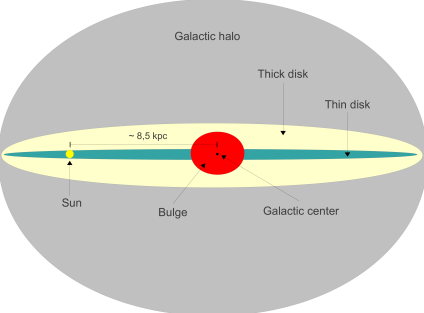
\includegraphics[width=0.5\textwidth]{image.png}
\caption{\label{fig:2}\emph{Thin and Thick disks in the Milky way}}
\end{figure}
There are far more stars in the thin disk, and as expected the younger stars are in the thin disc, where as the older ones are in the thick disk.
\item One can then combine the thick and thin disk in our density formula:
\begin{empheq}[box=\tcbhighmath]{equation}
\begin{split}
 n(R,z) = n_0(e^{-\frac{z}{h_{thin}}}+fe^{-\frac{z}{h_{thick}}})e^{-\frac{R}{h_R}}
\end{split}
\end{empheq}
Here $f<1$. This is only the disc density for stars, gases have different typically smaller scale heights. 


\end{itemize}
\subsection{Halo}
\begin{itemize}
    \item The Halo is the name given to the spherical structure that consist of stars, globular clusters, neutral gas and dark matter. The stars here are old so low metallicity($Z \leq 0.02Z_{\odot}$)
\end{itemize}

\subsection{The Bulge }
\begin{itemize}
    \item Located and the inner most 3kpc of the galaxy, it is dense with young stars that account for 20\% of the Galaxies light output. 
\end{itemize}

\subsection{The Bar} 
\begin{itemize}
    \item The Milky way also has a bar that extends out about 10kpc, from the galactic center.  
\end{itemize}
\subsection{Fermi Bubbles }
\begin{itemize}
    \item These are giant bubbles that extend above the galactic plane, emitting mostly gamma and a little X-ray radiation.  Open question to their origin but most likely a tidal disruption involving SgrA* swallowing a star. 
\end{itemize}

\subsection{Sgr A}
\begin{itemize}
    \item Sgr A is the brightest source in the Sagittarius system, is actually compromised of several sources, the brightest of them being the super massive black hole Sgr A*.

The mass of this black hole has been (semi) accurately determined by observing orbits of stars close to it. 
\end{itemize}

\subsection{Galactic Rotation}
\begin{itemize}
    \item All matter must be rotating around the galactic center, otherwise it would have simply fallen into the center. 

If we wish to measure the rotational velocities of other stars and objects, we must account for the fact that we ourselves are also rotating. This involves taking adding our own velocity vector to any measurement we see from the suns reference frame. 

We split the motion of other stars into two. The radial velocity is the velocity away or towards us, where as the transverse velocity is perpendicular to the radial velocity. 

Radial velocity results in red/blue shifting of the light emitted. 
\end{itemize}

\subsection{Oort constants}
\begin{itemize}
    \item These are empirically determined quantities that are related to properties of the Galaxies rotation.

Consider a star a distance $d$ from the sun, a distance $R$ from the GC and moving with velocity $V(R)$. Then also assume circular orbits and that the sun is located a distance $R_0$ from the GC and is moving with velocity $V_0$. 

Then the radial velocity can be expressed as:
\begin{empheq}[box=\tcbhighmath]{equation}
\begin{split}
V_r(R) = R_0\sin(l)\left(\frac{V}{R}-\frac{V_0}{R_0}\right)
\end{split}
\end{empheq}
Then we taylor expand the term in brackets for small ($R-R_0$) up to first order to obtain the following form for $V_r$:
\begin{empheq}[box=\tcbhighmath]{equation}
\begin{split}
 V_r(R) = Ad\sin(2l)
\end{split}
\end{empheq}
Where the first Oort constant $A$ is:
\begin{empheq}[box=\tcbhighmath]{equation}
\begin{split}
 A = -\frac{1}{2}\left(\left[\frac{dV}{dR}\right]_{R_0} - \frac{V_0}{R_0}\right)
\end{split}
\end{empheq}
\item In a similar manner for the transverse velocity we obtain the formula:
\begin{empheq}[box=\tcbhighmath]{equation}
\begin{split}
 V_t(R) = Ad\cos(2l)+Bd
\end{split}
\end{empheq}
Where $B$ is the second Oort constant:
\begin{empheq}[box=\tcbhighmath]{equation}
\begin{split}
 B = -\frac{1}{2}\left(\left[\frac{dV}{dR}\right]_{R_0} + \frac{V_0}{R_0}\right)
\end{split}
\end{empheq}
\item From measuring local stellar properties we can combine Oort constants to determine properties of the rotation curve of the Galaxy. 
\begin{empheq}[box=\tcbhighmath]{equation}
\begin{split}
 -A-B = \left[\frac{dV}{dR}\right]_{R_0} \\
A-B = \frac{V_0}{R_0}
\end{split}
\end{empheq}



\end{itemize}
\begin{figure}[H]
\centering
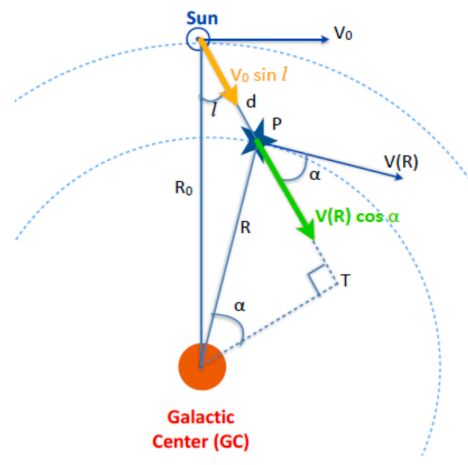
\includegraphics[width=0.6\textwidth]{Graph3.png}
\caption{\label{fig:2}\emph{Diagram for determining Oort constants}}
\end{figure}

\subsection{21cm Hydrogen line}
\begin{itemize}
    \item The anti-parallel spin states of the electrons in hydrogen have a slightly lower energy, though the parallel state is quite stable, half live $\approx 10^7$ years.  But with enough hydrogen you can of course see this. 

The 21cm line will naturally broaden from thermal activity. This has a width contribution of:
\begin{empheq}[box=\tcbhighmath]{equation}
\begin{split}
 \frac{\Delta f}{f} = \frac{8\ln (2)k_bT}{m_Hc^2}
\end{split}
\end{empheq}
The HI line is a great diagnostic tool. 

\end{itemize}

\subsection{Galactic rotation curve}
\begin{itemize}
    \item The measured Galactic rotation curve flattens out after a certain point. This is not however, what we would expect.  Based on the observable mass distribution after a certain point objects should be outside enough of the mass such that $M(R)$ does not grow with $R$. From that point on wards we get $V(R) = \sqrt{\frac{GM}{R}}$ so the rotation curve should decrease with R, not flat!

One way to "fix" this, is if the density $\rho(R) \propto R^{-2}$. This is is due to $\frac{dM}{dR} = 4\pi R^2\rho(R)$ This is not disc like, but in fact isotropic, leading to the term: dark matter halo. Some proposed models for dark matter density have arisen from N-body simulations of collision less dark matter and match the rotation curve, at least in simulations. 
\end{itemize}

\subsection{Galaxy groups} 
\begin{itemize}
    \item As we start to look at large scale structure in the universe we see that galaxies tend to be found in groups. 



\end{itemize}

\subsection{The Local group}
\begin{itemize}
    \item The group our galaxy is in is called the Local group. The Local group consists of 40+ galaxies 

\item There are three large galaxies that 90 \% of the Local groups light comes from. These are The milky way, Andromeda (M31) and Triangulum (M33). 

\item The approximate radius of the local group is $1 ~Mpc$. 
\end{itemize}

\subsection{Andromeda}
\begin{itemize}
    \item M31 is a bared spiral galaxy and is $\sim$  50\% more luminous, has a larger z height $6~kpc$ and higher metalicity. than the milky way. 

Has an isophotal radius of $46.6 ~kpc$
\end{itemize}

\subsection{Isophotal radius }
\begin{itemize}
    \item This is the distance to the isophote where B band magnitude drops to $25 mag/arcsecond^2$. This definition is independent of radius. 
\end{itemize}

\subsection{Triangulum}
\begin{itemize}
    \item M33 is a spiral galaxy \~ 20\% as bright as the milky way. 

It also has a large disk height of of $1.7 ~kpc$ but its disk is warped due to tidal interaction with M31. 

Has an isophotal disk height of $18.7~kpc$
\end{itemize}

\subsection{Magellanic clouds}
\begin{itemize}
    \item The Large  and Small Magellanic clouds (LMC and SMC), are two irregular dwarf galaxies. 

LCM has lots of star formation has the most active star forming region in the local group. 

SMC has much recent star formation and many high mass stars and X-ray binaries. 
\end{itemize}

\subsection{Tidal Streams}
\begin{itemize}
    \item Dwarf galaxies orbiting much more massive central galaxies can be disrupted. 

This disruption leaves behind streams indicating the orbital trajectories even long after the galaxies have been ripped apart. 

\item Tidal forces arise due to different gravitational forces. The 

change in gravitational force going from $r$ to $r+ \Delta r$ is given by: 
\begin{empheq}[box=\tcbhighmath]{equation}
\begin{split}
\Delta f_{Tide} = \frac{d f}{dr}\Delta r
\end{split}
\end{empheq}
Then since we know $F = \frac{GMm}{r^2}$:
\begin{empheq}[box=\tcbhighmath]{equation}
\begin{split}
 F_{Tide} = \frac{-2GMm}{r^3}\Delta r
\end{split}
\end{empheq}
Thus falls of as $r^{-3}$, not $r^{-2}$ like gravity. 



\end{itemize}

\subsection{Jacobi radius (Roche Limit)}
\begin{itemize}
    \item This is the distance from the center of a Satellite where the Tidal forces from the central galaxy are equal to the Gravitational forces of the satellite:
\begin{empheq}[box=\tcbhighmath]{equation}
\begin{split}
r_j = R \left( \frac{M_{Sat}}{2M_{CG}}\right)^{\frac{1}{3}}
\end{split}
\end{empheq}
There is a problem called the missing satellite problem as there are predicted to be 50 times more galaxies in the local group then currently visible. 

This could be solved by super faint galaxies that are full of dark matter!
\end{itemize}

\subsection{Properties of different types of galaxies}
\subsubsection{Spiral galaxies}
\begin{itemize}
    \item The spiral arms of these galaxies are described as "blue" meaning the magnitude of the light coming from the blue band $B$ is lower (more light) thus we say $B-V<1$. This corresponds to active star formation in these regions. 

The bulge of these galaxies is more yellow/red, written as $B-V >1$, this means there is no star formation "red and dead".  

\item We can conclude that these galaxies contain stars, gas, dust and dark matter. Star formation will continue here and the galaxies rotating disc was most likely formed via gas collapse. The presence of globular clusters also indicate that merging may have been part of the formation process. 

These galaxies have typical absolute magnitudes in the range of $-21< M_V < -17$, they are thus relatively high mass galaxies.  The spectra of these galaxies contain absorption lines which come from stars and emission lines which come from hot gas. 
\end{itemize}

\subsubsection{Elliptical galaxies}
\begin{itemize}
    \item Elliptical galaxies have a smooth brightness profile, they have little to no dust or gas as their spectra show absorption lines only. Also have many globular clusters. The galaxies are not rotating as a whole. They have typical absolute magnitudes in the range of $-22<M_V < -18$

\item Elliptical are considered "Red" as they have $B-V >1$, thus an old stellar population, with a high surface brightness meaning stars are densely packed. No ongoing star formation as there is no gas. The lack of rotation implies formation via merger. They are typically more massive then spiral galaxies.
\end{itemize}

\subsubsection{Irregulars}
\begin{itemize}
    \item Typically blue $B-V<0.8$, they have a low surface brightness and are highly asymmetrical. These galaxies have a lot of dust and show strong emission lines.  Absolute magnitude of $-18 < M_V < -10$, these galaxies also rotate.  These are young galaxies whose structures are still forming . They also have few globular clusters meaning they are formed during collapse. 
\end{itemize}

\subsection{The continuum}
\begin{itemize}
    \item The spectra of galaxies is made up of many different blackbody spectra, as the temperature of a body decreases its spectra tends to have a lower amplitude and the peak wavelength gets longer.  However as we know from the mass distribution function there are far more stars with lower temperature then higher. These two effects cancel each other out so that the over all spectrum of the galaxy flattens out with wavelength. 
\end{itemize}



\begin{figure}[H]
\centering
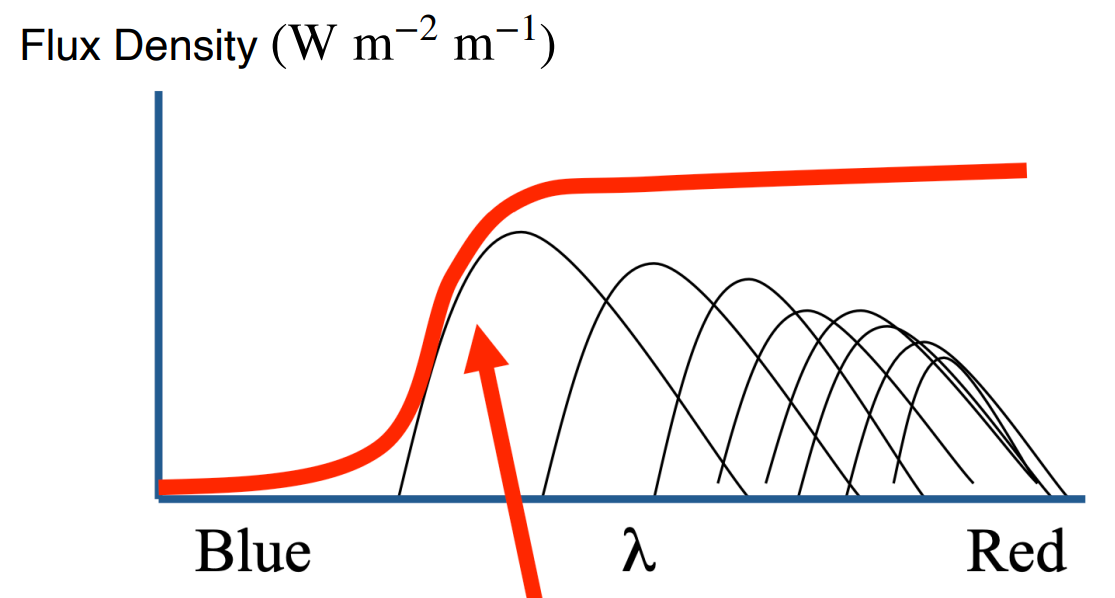
\includegraphics[width=0.6\textwidth]{Graph4.png}
\caption{\label{fig:2}\emph{Flattening out of a galaxies spectrum}}
\end{figure}
\begin{itemize}
    \item What we can also see from this graph is that below a certain wavelength (4000 Angstrom) there is pretty much no flux density, this is just due to the lack of stars that are that hot (i.e. that big). This is known as the 4000 Angstrom break. 
\end{itemize}

\subsection{Absorption and emission lines}
\begin{itemize}
    
 \item Absorption can also happen due to cold gas. Absorption always involves the absorption of a photon with an electron going to a higher energy level and staying there , releasing no other photons. 

\item Emission occurs as atoms are ionised, heated and re-emit at a different wavelength. This often occurs in an area with on going star formation. This requires very hot type O/B stars. 

\end{itemize}

\subsection{Redshift}
\begin{itemize}
    \item Is the quantity $z$ that measures how Doppler shifted something is due to its motion with respect to the rest frame of the galaxy. $z$ is given by:
\begin{bux}
    \begin{split}
        z = &\frac{\lambda_{obs}-\lambda_{em}}{\lambda_{em}} = \sqrt{\frac{(1+v/c)}{(1-v/c)}} \\
 & \text{for}~~ v<<c,~~~z = \frac{v}{c}
     \end{split}
\end{bux}
\end{itemize}


\subsection{Surface Brightness}
\begin{itemize}
    \item This is a measure of the intensity in a region of the sky. It is defined as: 
\begin{bux}
    \begin{split}
        I =\frac{F}{\alpha^2}
    \end{split}
\end{bux}
Here $F=L/4\pi d^2$ is the flux and $\alpha$ is the angular area, so angular size $D$ over the distance $d$ squared  $\alpha = \frac{D^2}{d^2}$. This means that this intensity is independent of  distance! (at least for local universe) 
\begin{bux}
    \begin{split}
        I = \frac{L}{4\pi D^2}
    \end{split}
\end{bux}
This is also a good way to calculate luminosity. However on larger scales due to the concept of distance changing at large Redshift's this is not quite the case.  Surface brightness is measured in units of $L_{\odot}/pc^2$ or $mag/acrsec^2$. 

\item In practise the radial profiles of brightness are measured, i.e. average brightness at a given distance $r$ from the center. The "sky background" also has its own brightness of $21.8~mag/arcsec^2$. 

\item In spiral galaxies there are two components to the brightness, from the disk and from the bulge. The disk follows the exponential profile: 
\begin{bux}
    \begin{split}
        I(r) = I_0e^{-\frac{r}{h_r}}
    \end{split}
\end{bux}
Where as the bulge follows as "Sersic profile":
\begin{bux}
    \begin{split}
        I(r) = I_0e^{-(\frac{r}{R_0})^{\frac{1}{n}}}
    \end{split}
\end{bux}
\item Ellipticals also have a general Sersic profile: the same as above but it is sometimes recast as:
\begin{bux}
    \begin{split}
        I(r) = I_0e^{-b(\frac{r}{R_0})^{\frac{1}{n}}-1}
    \end{split}
\end{bux}
Where the parameter $b$ is chosen so that the circle with radius $R_e$ contains half the light of the galaxy. many ellipticals follow a Sersic profile with $n=4$ this is known as a de Vaucoulers profile.

\item To determine the luminosity $L$, from this profile we just have to integrate over $r$  and the azimuthal angle $\phi$:
\begin{bux}
    \begin{split}
        L = \int_0^{2 \pi}\int_0^{\infty}I(r,\phi)rdrd\phi
    \end{split}
\end{bux}
If we do this for the Sersic profile along with the substitution $x = (\frac{r}{R_0})^{\frac{1}{n}}$ then: 
\begin{bux}
    \begin{split}
           L =I_0 \int_0^{2 \pi}\int_0^{\infty}x^nR_0nx^{n-1}R_0e^{-x}dxd\phi = 2\pi I_0R_0^2n\int_0^{\infty}x^{2n-1}e^{-x}dx
    \end{split}
\end{bux}
The last integral here can be recognised as the gamma function $\Gamma(m)$ for $m=2n$. So:  
\begin{bux}
    \begin{split}
        L = 2 \pi I_0R_0^2n\Gamma(2n) = \pi I_0R_0^2(2n)!
    \end{split}
\end{bux}
Where the last step only holds if $n$ is a natural number. One could also do this calculation in terms of the half light radius $R_e$ and surface brightness at this distance $I_e$. With this method and $n=4$ as mentioned, the resulting luminosity is:
\begin{bux}
    \begin{split}
        L = 7.22\pi I_eR_e^2
    \end{split}
\end{bux}

\end{itemize}

\subsection{Luminosity function}
\begin{itemize}
    \item Just as with the mass function we can create a function that tells us the amount of galaxies there are at a certain luminosity.  This is defined as the quantity $\phi$ such that:
\begin{bux}
    \begin{split}
        \phi = \frac{dn}{dL}
    \end{split}
\end{bux}
Where $n$ is number of galaxies. This quantity has units $\text{galaxies}/Mpc^3 \text{per unit luminosity interval}$.  When we take into account that our samples are flux limited, i.e. we cannot see  galaxies below a certain point we arrive at the following luminosity function: 
\begin{bux}
    \begin{split}
        \phi(L) = \frac{\phi_{\ast}}{L_{\ast}}e^{-\frac{L}{L_{\ast}}}\left( \frac{L}{L_{\ast}}\right)^{\alpha}
    \end{split}
\end{bux}
Here $\phi_{\ast}$ is a normalisation constant that is well measured and $L_{\ast} \approx 2 \times 10^{10}L_{\odot}$, is the characteristic luminosity, that is the point at which the function changes from power law to exponential. This is a Schechter function. 
\end{itemize}


\subsection{Stellar dynamics}
\begin{itemize}
    \item We expect two stars a distance $D$ apart, with a relative velocity $V$ and for the sake of simplicity the same mass $M$ to have a strong encounter when the gravitational energy between them $U$ is greater then the relative kinetic energy $K$. This happens when:
\begin{bux}
    \begin{split}
       & \frac{GM^2}{D} \geq \frac{MV^2}{2} \\
    \implies & D \leq \frac{2GM}{V^2}
    \end{split}
\end{bux}
This radius of strong encounters $D_{max}= \frac{2GM}{V^2}$ sweeps out a volume $\mathcal{V} = \pi D_{max}^2Vt$ in a time $t$. Here we have considered every other star fixed with a velocity $0$. If the number density of stars is $n$ then the number of strong encounters is: 
\begin{bux}
    \begin{split}
        N = \int nd\mathcal{V} = n\mathcal{V} = \frac{4\pi n G^2M^2t}{V^3}
    \end{split}
\end{bux}
The average time to have one strong encounter is then when $N=1$. If we put in reasonable numbers for stars in galaxies, the time $t$ that results in $N=1$ is larger then the age of the Universe, so we can treat stars in galaxies as collision-less gas. 
\end{itemize}

\subsection{Tully-Fisher Relation}
\begin{itemize}
    \item This is an empirically observed correlation between luminosity of a spiral galaxy and its asymptotic maximum rotational velocity.  From equating centripetal force to the gravitational force we can see that the mass enclosed in a radius $r$ is related to the velocity at that radius by: 
\begin{bux}
    \begin{split}
        M(r) = \frac{V^2r}{G}
    \end{split}
\end{bux}
If we assume that all spiral galaxies have the same surface brightness $I \propto L/r^2$ and if we assume that all spiral galaxies have the same mass-to-luminosity ratio then $M(r) \propto L \propto r^2$.  Thus $ L \propto V_{max}^2\sqrt{L}$ so: 
\begin{bux}
    \begin{split}
        L \propto V_{max}^4
    \end{split}
\end{bux}
This is a rough sketch of why the Tully-Fisher relationship exists. 
\end{itemize}

\subsection{Virial theorem}
\begin{itemize}
    \item This equation can be derived from imposing hydrostatic equilibrium on the Naiver stokes equations. The result is: 
\begin{bux}
    \begin{split}
        \frac{1}{2}\ddot{I} = 2T + 2U + \Omega + M_B
    \end{split}
\end{bux}
Here $I$ is the moment of inertia, so $\frac{1}{2}\ddot{I}$ is the is the total rotational energy. $T$ is the total kinetic energy. $U$ is the total thermal energy, $\Omega$ is the total gravitational energy and $M_B$ is the total magnetic pressure. 

In a molecular cloud $\ddot{I} \approx U \approx 0$ so:
\begin{bux}
    \begin{split}
        2T + \Omega + M_B = 0
    \end{split}
\end{bux}
Where as in main sequence stars, we examine from a reference frame that is not moving or rotating as well as negligible magnetic field so:
\begin{bux}
    \begin{split}
        2T + \Omega =0
    \end{split}
\end{bux}

In galaxies there are stable orbits $\ddot{I} =0 $ small magnetic fields, so $M_B=0$ and the density of gas is small so $U=0$. This leads to: 
\begin{bux}
    \begin{split}
        2T + \Omega = 0
    \end{split}
\end{bux}
\end{itemize}

\subsection{Dynamics in Ellipticals}
\begin{itemize}
    \item There is no organised motion of stars here, only random 
    velocity vectors. We can characterise the system with the velocity dispersion $\sigma$. This is just the standard deviation of velocity about the mean velocity.  This can be measured by looking at the broadening of spectral lines.

In $1$-D  the standard deviation of the lines is the velocity so $\sigma = V_{1D}$, In $3$-D from spherical symmetry $V_{3D}^2= 3\sigma^2$. So:
\begin{bux}
    \begin{split}
        2T = \int v^2dm = 3M\sigma^2
    \end{split}
\end{bux} 
And the total gravitational energy:
\begin{bux}
    \begin{split}
        \Omega = -\int_{center}^{surface}\frac{GM(r)dm}{r} = -\frac{3}{5}\frac{GM^2}{R}
    \end{split}
\end{bux}
So by the Virial theorem:
\begin{bux}
    \begin{split}
        M_{vir} = \frac{5\sigma^2R}{G}
    \end{split}
\end{bux}
Or more simply $M_{vir} \propto \sigma^2R_{e}$, where $R_{e}$ is the half light radius.  If we use the fact that galaxies have a constant mass to luminosity ratio then $(M/L)L \propto \sigma^2R_e$ so $L \propto \sigma^2R_e$. Also we know the measured surface brightness is $L \propto I_eR_e^2$. Thus:
\begin{bux}
    \begin{split}
       & L \propto \sigma^2(L/I_e)^{\frac{1}{2}} \\
& \implies L \propto \sigma^4
    \end{split}
\end{bux}
Also: 
\begin{bux}
    \begin{split}
        R_e \propto \sigma^2/I_e
    \end{split}
\end{bux}
This last relation tell us the 3rd of these relations if we know the other 2. Thus in the $3$-D parameter space all galaxies lie on a $2$-D plane. This is called the fundamental plane of galaxies. 
\end{itemize}

\begin{figure}[H]
\centering
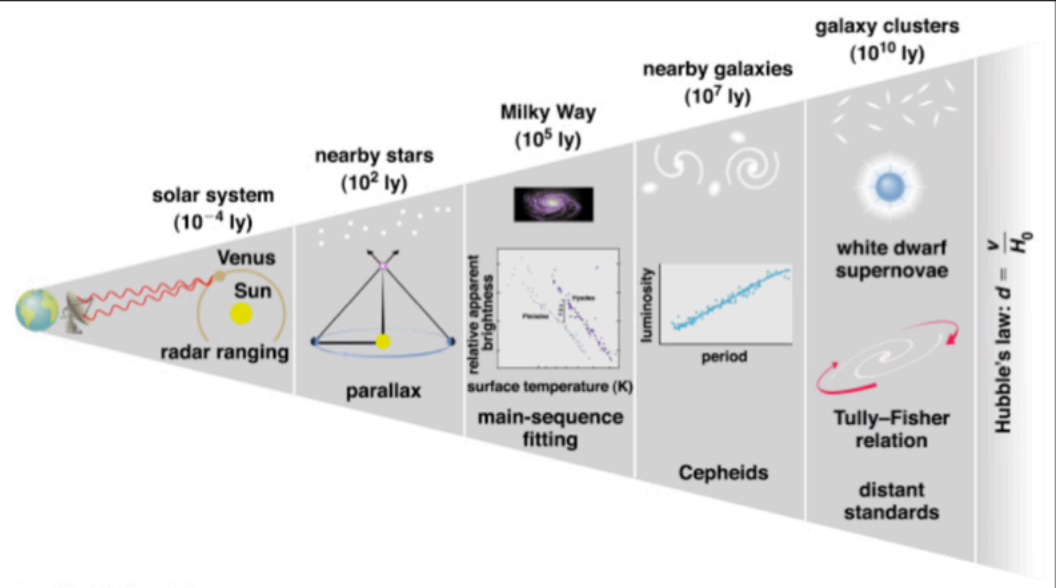
\includegraphics[width=0.8\textwidth]{Graph5.png}
\caption{\label{fig:2}\emph{Cosmic distance ladder}}
\end{figure}

\subsection{Galaxy spectra}
\begin{itemize}
\item Elliptical galaxies are characterised by strong absorption lines, due to metals in the stellar atmospheres of the low luminosity stellar population. Few emission lines as there is essentially no young stars and no gas. 
\begin{figure}[H]
\centering
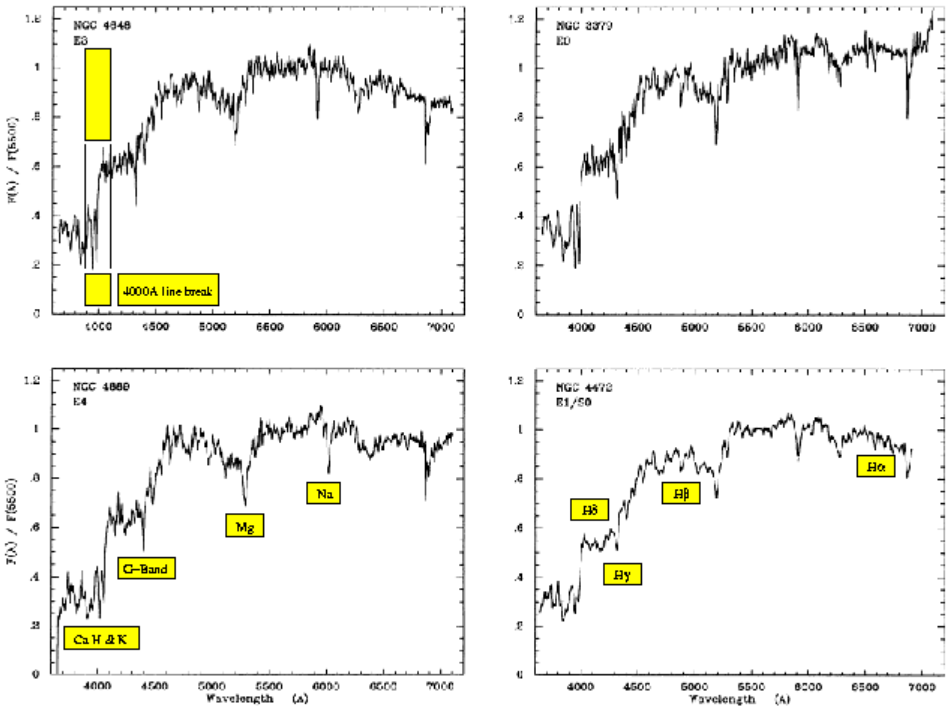
\includegraphics[width=0.8\textwidth]{Graph6.png}
\caption{\label{fig:2}\emph{Elliptical spectra}}
\end{figure}
\item Spiral Galaxies are characterised by strong emission lines due to hot young stars which heat the surrounding gas, and by absorption features due to the older, underlying stellar population 

\begin{figure}[H]
\centering
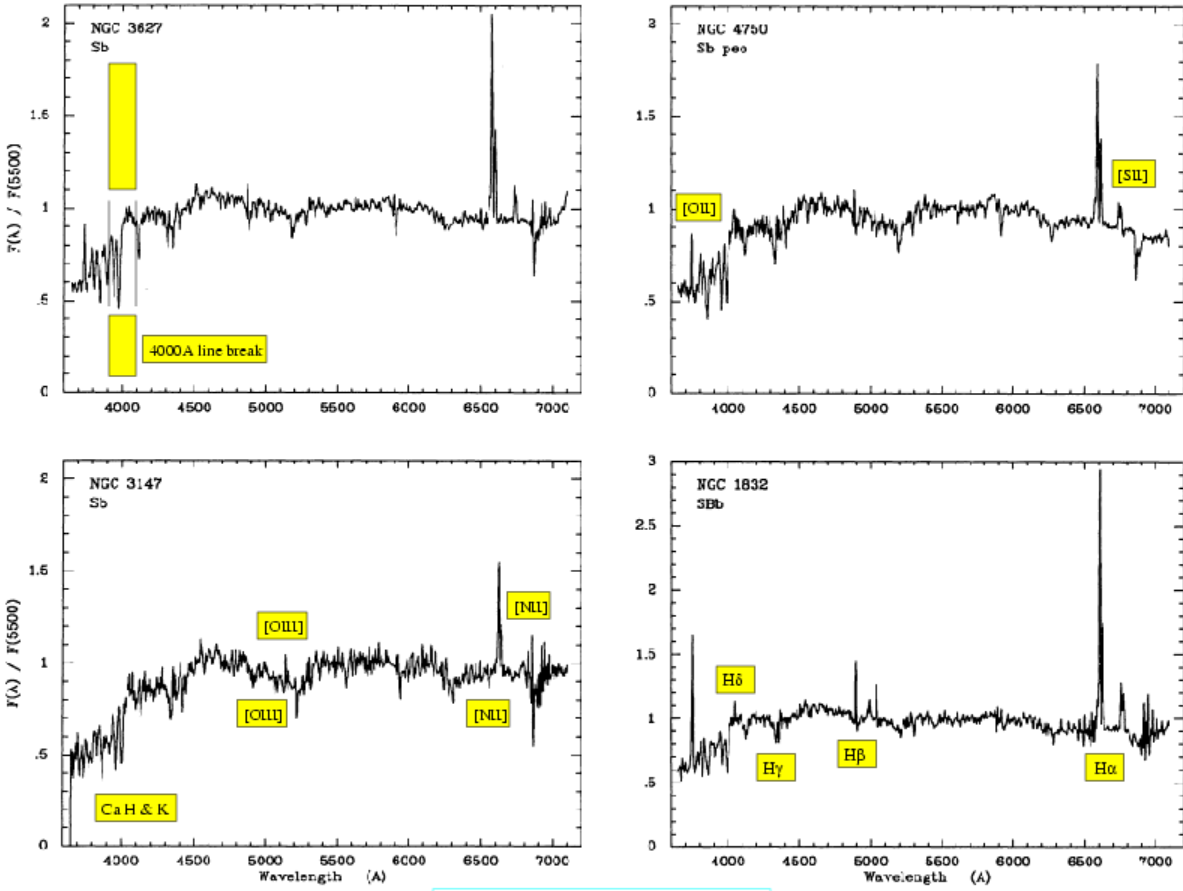
\includegraphics[width=0.8\textwidth]{Graph7.png}
\caption{\label{fig:2}\emph{Spiral spectra}}
\end{figure}

\item Irregular galaxy spectra are characterized by strong emission lines, due to hot young stars and surrounding HII regions.  the 4000 anstrom break is also not very prevelenet here as they dont have enough metals to absorb at this point and younger stars mean higher abundance of Type O and B stars that are bigger and hotter. 

\begin{figure}[H]
\centering
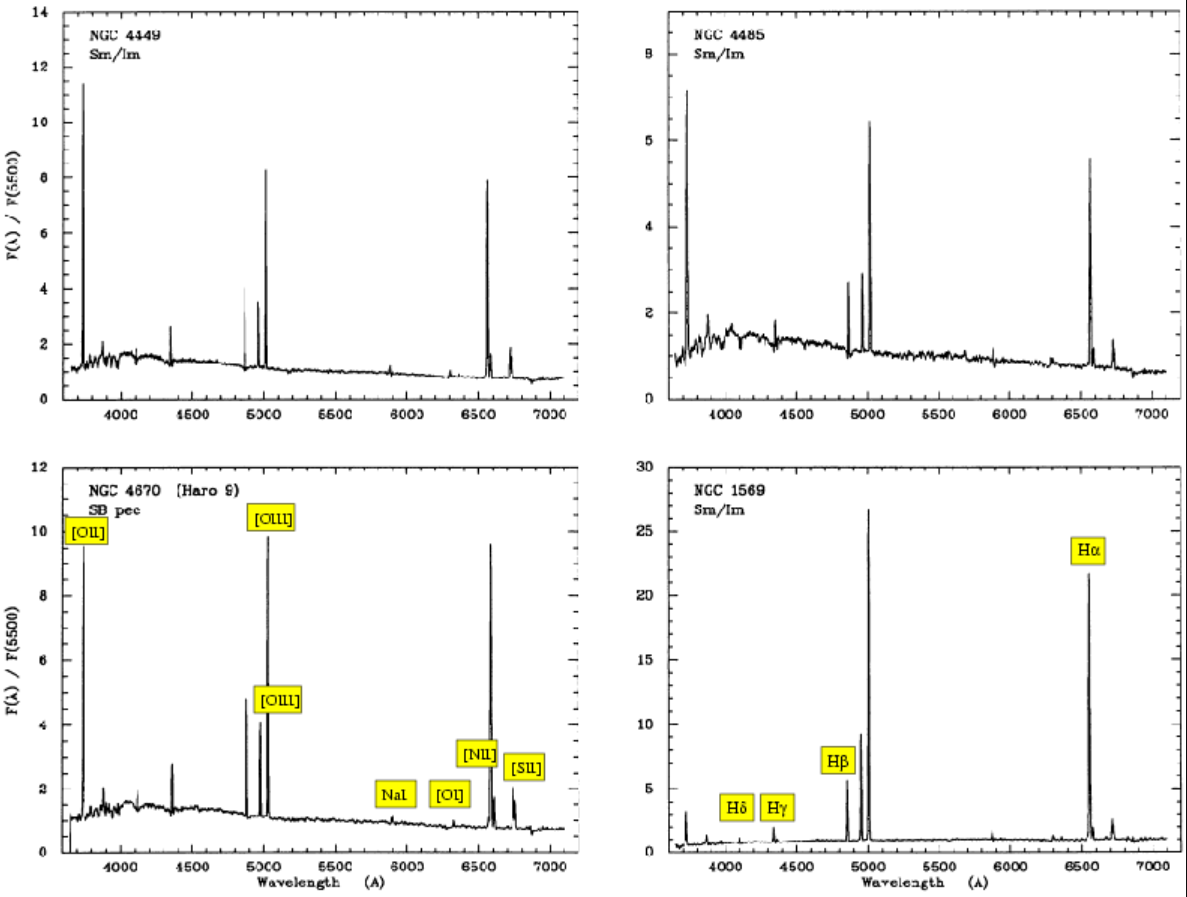
\includegraphics[width=0.8\textwidth]{Graph8.png}
\caption{\label{fig:2}\emph{Irregular galaxy spectra}}
\end{figure}
\end{itemize}


Source: \url{http://astronomy.nmsu.edu/nicole/teaching/ASTR505/lectures/lecture26/slide01.html#:~:text=Spiral%20galaxy%20spectra%20are%20characterized,the%20older%2C%20underlying%20stellar%20population.&text=Irregular%20galaxy%20spectra%20are%20characterized,stars%20and%20surrounding%20HII%20regions.}
\end{document}


